\thispagestyle{fancy}

\newpage
\section{Optische Polarisation und Valenzbandstuktur}
\label{chap:polgrund}
%
Durch die Prozessierung und die Flip-Chip-Montage kann Licht nur durch die untere, unbewachsene Seite des Saphir-Substrates ausgekoppelt werden. Die Art und Weise der Lichtauskopplung hat einen bedeutenden Einfluss auf die EE und damit auf die EQE. Durch die Geometrie bestimmt, hängt die EE maßgeblich vom Emissionsprofil ab, sodass Licht, welches senkrecht zur Quantenfilmebene abgestrahlt wird, die höchste EE aufweist. Um diese zu optimieren, ist es wichtig, die Bandstrukturen zu betrachten.
\begin{figure}[H]
    \centering
    \begin{minipage}[t]{0.49\linewidth}
        \centering
        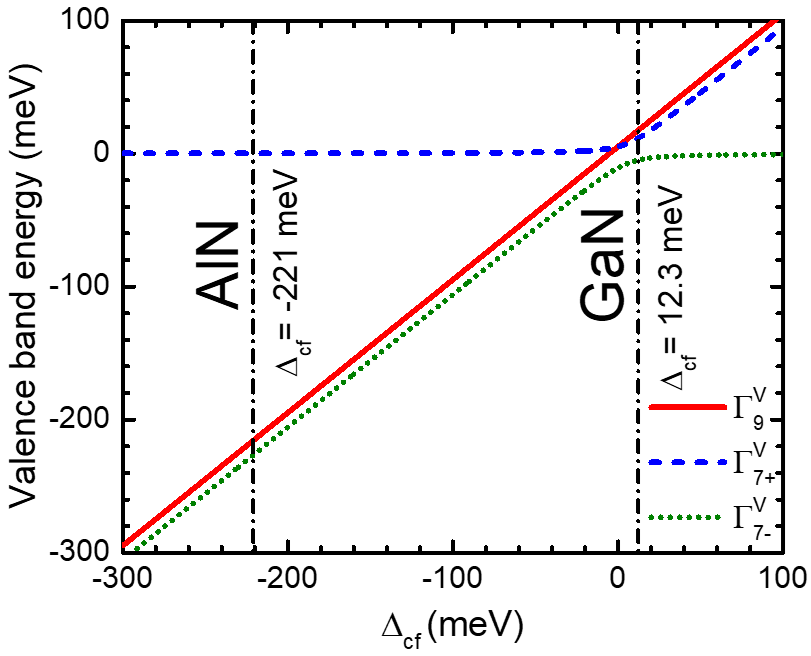
\includegraphics[width=\linewidth]{Bilder/vancebandPlot.png}
        \caption{Energetische Reihenfolge der Valenzbänder in Abhängigkeit der Kristallfeldaufspaltung. Sichtbar ist der Wechsel der Bandanordnung mit sinkender Kristallfeldaufspaltung und der Effekt des "`anti-crossing"' bei den Bändern gleicher Symmetrie. \cite{doi:10.1063/1.4932651}    }
        \label{fig:auger5k}
    \end{minipage}% <- sonst wird hier ein Leerzeichen eingefügt
    \hfill
    \begin{minipage}[t]{0.49\linewidth}
        \centering
        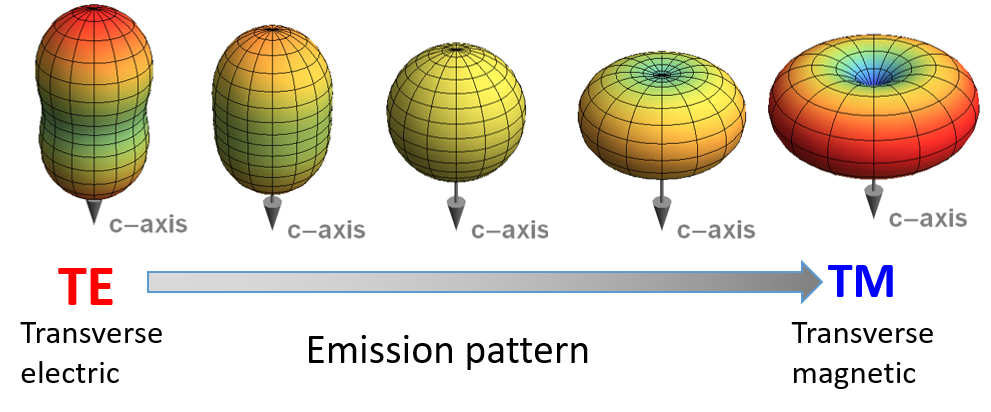
\includegraphics[width=\linewidth]{Bilder/martinTETM.png}
        \caption{Kontinuierlich ändernde Abstrahlcharakteristik in Abhängigkeit der Polarisation von TE- zu TM~\cite{martingut}.  }
        \label{fig:martintetm}
    \end{minipage}
\end{figure}
\vspace{0.1cm}
\noindent
Die Valenzbandstrukturen von AlN und GaN unterscheiden sich durch die unterschiedliche Anordnung der Bänder. Neben dem Leitungsband gibt es ein durch Spin-Bahn-Wechselwirkung und Kristallfeldenergie dreifach aufgespaltenes Valenzband~\cite{doi:10.1063/1.117689}. Sie werden nach ihrer energetischen Lage als A-,B- und C-Band bezeichnet. In AlN hat das A-Band eine $\Gamma^{L}_{7+}$, das B-Band eine $\Gamma^{L}_{9}$ und das C-Band eine $\Gamma^{L}_{7}$ Symmetrie. Bei GaN hingegen gilt folgende Reihenfolge:  $\Gamma^{L}_{9}$, $\Gamma^{L}_{7+}$, $\Gamma^{L}_{7}$. Die Ursache für den Symmetriewechsel liegt in der großen negativen Kristallfeldenergie von AlN mit einem Wert von $-221 \thinspace meV$ \cite{PhysRevB.87.235209} im Vergleich zur positiven von GaN mit $12,3 \thinspace meV$ ~\cite{PhysRevB.81.155202}. Bei Raumtemperatur wird, nach der Fermi-Dirac-Verteilung, das oberste Band mit der $\Gamma^{L}_{7+}$-Symmetrie besetzt. Aus Zuständen des $p_z$ bestehend wird transversal magnetisch (TM) polarisiertes Licht emittiert. Die strahlende Rekombination findet demnach überwiegend mit Elektronen und Löchern aus dem A-Band mit $\Gamma^{L}_{7+}$-Symmetrie statt.
\begin{figure}[htb]
  \centering
  \begin{minipage}{\linewidth}
      \centering
        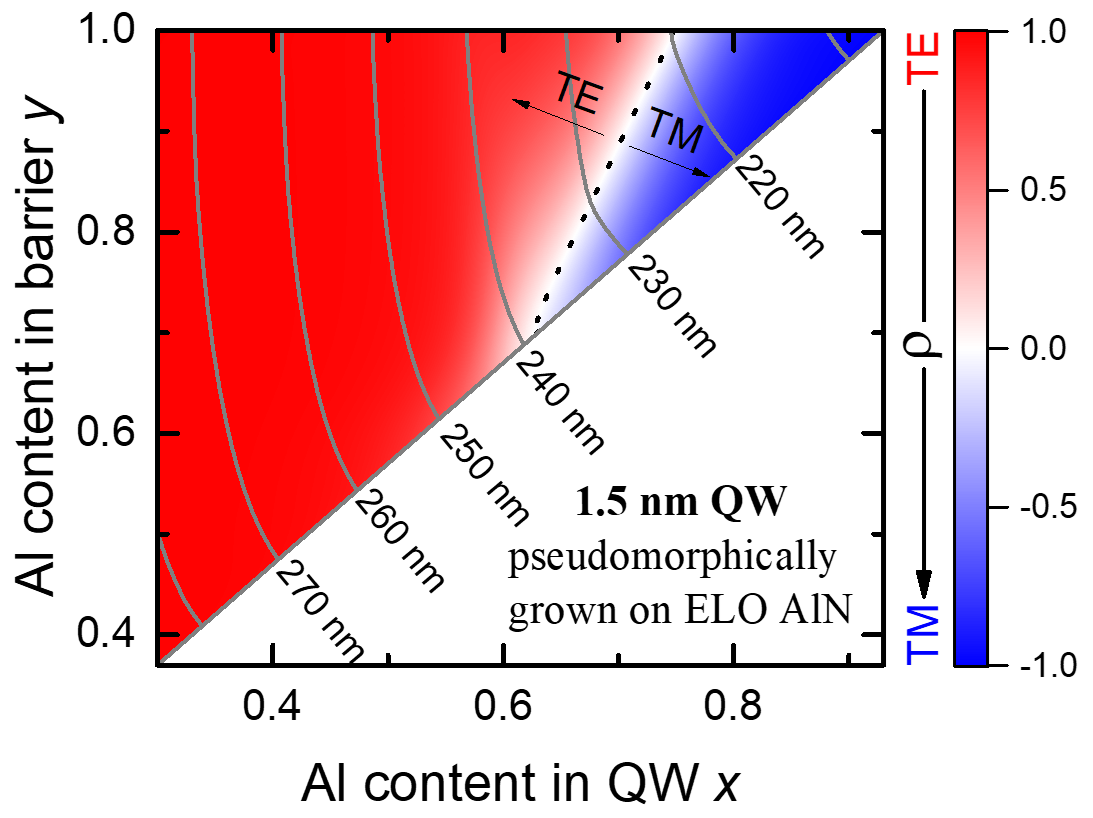
\includegraphics[width=0.6\textwidth]{Bilder/christophPolarisationSimu.png}
      \caption{Simulationsergebnisse des Polarisationsgrades in Abhängigkeit der Aluminiumkonzentration der Barrieren und QWs, basierend auf
dem k·p-Modell, für AlGaN-QW mit $1.5nm$-Dicke, die pseudomorph auf ELO-AlN gewachsen wurden. Die gestrichelte Linie zeigt, dass der Wechsel der Polarisation vom Aluminiumanteil in den Barrieren und QWs abhängig ist \cite{doi:10.1063/1.4932651}.}
      \label{fig:simuchr}
  \end{minipage}
\end{figure}
\noindent
\newline
In GaN ist das oberste Valenzband am $\Gamma$-Punkt mit $\Gamma^{L}_{9}$-Symmetrie. Das elektrische Feld des Lichtes ist senkrecht zur c-Kristallachse und wird durch Übergänge ins A- und B- Band erzeugt~\cite{doi:10.1063/1.3574025}, die aus Zuständen des $p_x$-und $p_y$-Orbitals bestehen. Bei strahlender Rekombination von Elektronen mit den Löchern im A- und B-Band entsteht also überwiegend TE-polarisiertes Licht ~\cite{doi:10.1063/1.3574025} . 
%
\begin{figure}[ht!]
  \centering
  \begin{minipage}{\linewidth}
      \centering
      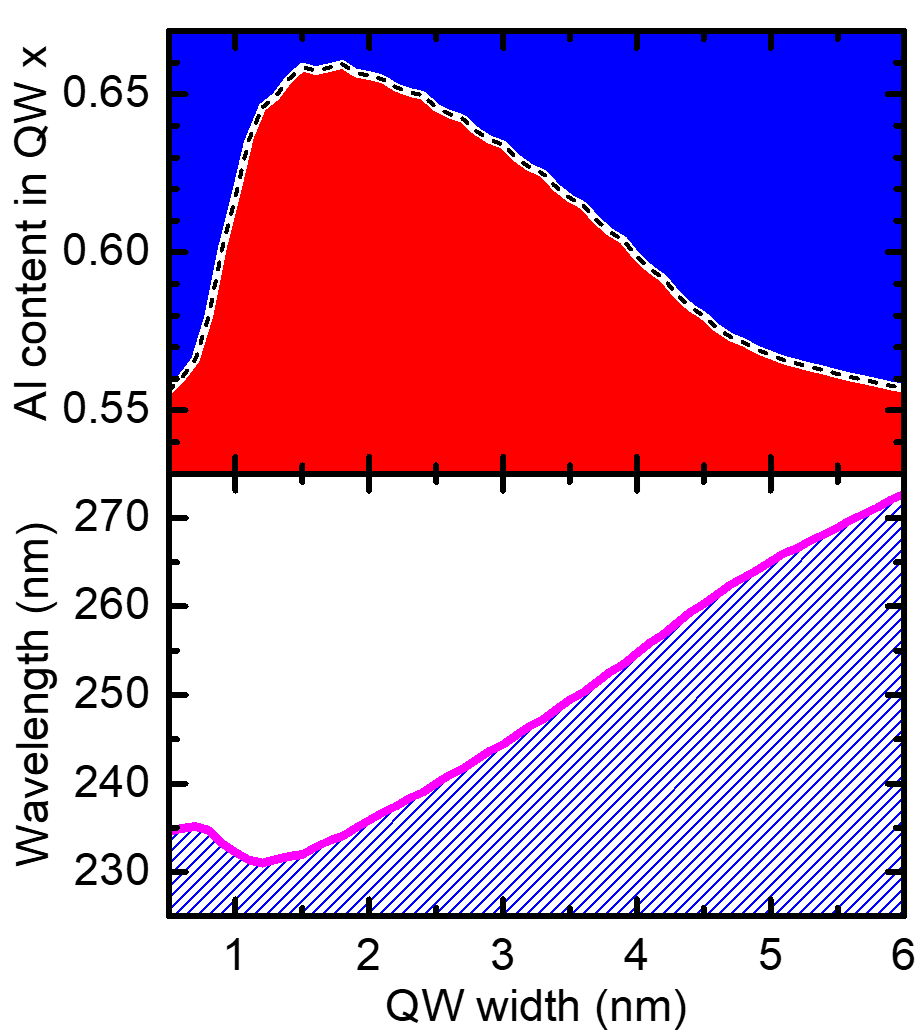
\includegraphics[width=0.6\linewidth]{Bilder/christophPolarisationSimu1.png}
      \caption{Ergebnisse der Simulation für die Polarisation in Abhängigkeit von der QW-Dicke(Wellenlänge) und dem Al-Gehalt in den QWs ~\cite{doi:10.1063/1.4932651}.}
      \label{fig:simu1chr}
  \end{minipage}
\end{figure}
%
Licht kann nicht ausgekoppelt werden, da es nur in der x-y- Ebene (parallel zur Quantenfilmebene) emittiert. Daraus resultierend sinkt die EE und damit die EQE. Bei $Al_{x}Ga_{1-x}N$ kommt es mit steigendem Aluminiumgehalt zu einer kontinuierlichen Verschiebung der Valenzbänder. Folgend tritt das sog. "`anti-crossing"' des $\Gamma^{L}_{7+}$ und $\Gamma^{L}_{7-}$ auf und resultiert in einer Änderung der Oszillatorstärke und folglich der Polarisationseigenschaften ~\cite{doi:10.1063/1.4932651}.
\newline
Das bedeutet, dass die Lichtemission sich hauptsächlich von TE-polarisiertem Licht zu TM-polarisiertem Licht ändert. Der genaue Aluminiumgehalt, an dem die Valenzbandkreuzung auftritt, ist noch nicht hinreichend bekannt. Theoretische Betrachtungen sagen für unverzerrtes $Al_{x}Ga_{1-x}N$ einen Kreuzungspunkt bei ca. $7\%$ vorher ~\cite{doi:10.1063/1.3675451}. Durch den starken Einfluss von Verzerrungen auf die Energie der  Valenzbandkante, ist die Polarisation von der wachsenden biaxialen Verzerrung bei steigendem Aluminiumgehalt abhängig. So wurde von Kawanishi et al. experimentell der Wechsel bei einem Aluminiumgehalt von "`75\%"' festgestellt \cite{doi:10.1063/1.2410242}. 
Noch dazu ist die Polarisation bei MQWs vom Ladungsträgereinschluss abhängig. Dieser ist hauptsächlich durch die Barrierenhöhe und Barrierendicke bestimmt. Mit kleiner werdender Barrierendicke steigt durch den gesteigerten Einfluss des QCSE der Grad der Polarisation \cite{PhysRevB.84.035305}. 
\newline
Reich et al. untersuchte unter diesem Zusammenhang die optische Polarisation der Emission von UVC-Leuchtdioden(LEDs) auf Basis von (0001) orientierten $Al_{x}Ga_{1-x}N$-MQWs mit Simulationen und Elektrolumineszenzmessungen ~\cite{doi:10.1063/1.4932651}. Dabei stellte er fest, dass mit zunehmendem Aluminium-Gehalt in den QWs die inplanare-Intensität des TE polarisierten Lichtes gegenüber dem des TM polarisierten Lichts abnimmt, was auf die Neuordnung der Valenzbänder in $Al_{x}Ga_{1-x}N$ zurückzuführen ist. 
\newline
Durch Modellrechnungen, basierend auf dem  \textbf{k$\cdot$p}-Modell, wurde die Abhängigkeit der Polarisation von der Aluminiumkonzentration in den Barrieren und QWs für pseudomorph aufgewachsenes ELO-AlN, wie Abbildung \ref{fig:simuchr} zeigt, berechnet. Zusätzlich wurde die Polarisation in Abhängigkeit einer Variation der QW-Dicke und dem Al-Gehalt in den QWs, wie in Abbildung \ref{fig:simu1chr} sichtbar, betrachtet.
\begin{figure}[ht!]
  \centering
  \begin{minipage}{\linewidth}
      \centering
      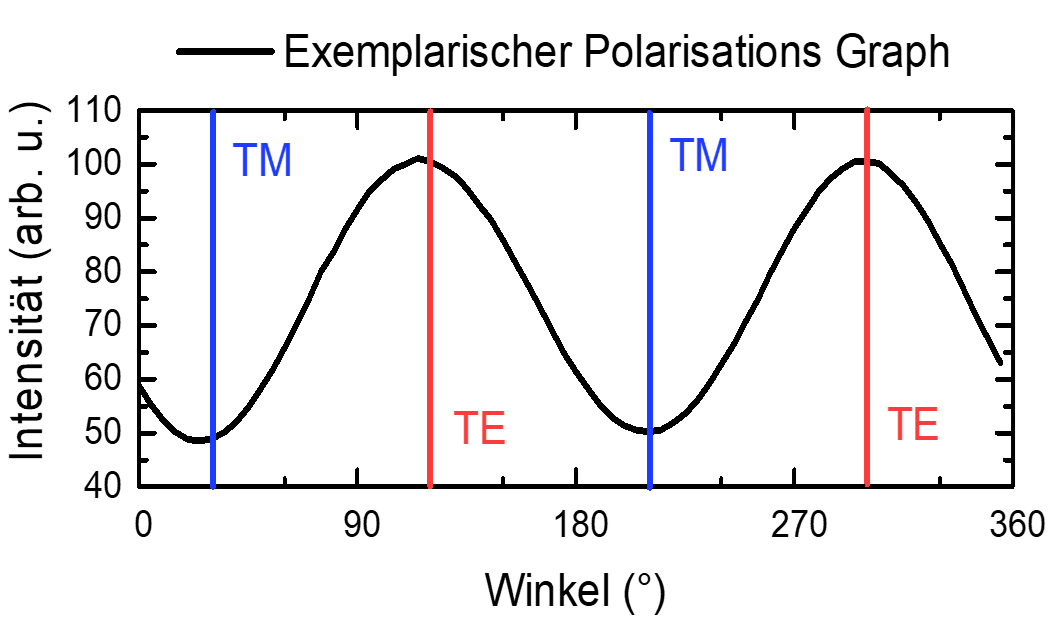
\includegraphics[width=0.6\linewidth]{Bilder/exemplPolGraph.png}
      \caption{Exemplarischer Graph einer Polarisationsmessung mit Hilfe von Photolumineszenzspektroskopie. Zu sehen ist die integrierte Intensität in Abhängigkeit des Winkels eines Polarisators. Zur Bestimmung des Polarisationsgrades wird die integrierte Intensität der TM-Emission(Blau) $I_{T;}$  und der TE-Emission(Rot) $I_{TE}$ in Gleichung ~\ref{eq:pol} eingesetzt.}
      \label{fig:degra}
  \end{minipage}
\end{figure}
Diese Erkenntnisse lassen sich zusätzlich mit Hilfe von Photolumineszenz prüfen. So lässt sich die Polarisation ermitteln, indem die Polarisation $\rho$ der Photolumineszenzemission aus der Kante einer Probe mit Hilfe der Gleichung 
\begin{equation}
\rho = \frac{ I_{TE} - I_{TM} }{ I_{TE} - I_{TM} } 
\label{eq:pol}
\end{equation}
bestimmt wird. Dabei ist $I_{TE}$ die integrierte Intensität der TE-polarisierten und $T_{TM}$ die Intensität der TM-polarisierten Emission. 
 


